\sectionframe{Original Model}

\section{Original Model}

\begin{frame}{Original Model Problem Domain}
    Power Converter DC $\to$ AC.
    Types:
    \begin{itemize}
        \item fixed frequency (stroboscopic mapping, continuous)
        \item variable frequency (first return mapping, discontinuous)
              \hspace{2em}
              \raisebox{-.7em}{
\includegraphics[height=2em]{gfx/you_are_here.png}}
    \end{itemize}

    \pause
    \vspace{2em}
    Model maps
    \begin{itemize}
        \item Input: Point at which the converter switched the last time $\theta \in [0, 2 \pi)$
        \item Ouput: Point at which the converter will switch the next time $F(\theta) \in [0, 2 \pi)$
    \end{itemize}
\end{frame}

\begin{frame}{Original Model (1/3)}
    \vspace{-2.0em}
    \begin{align}
        \theta      & \mapsto  F(\theta) \mod 2 \pi
        \\
        F(\theta)   & = \begin{cases}
                            F_1(\theta) & \text{if } q \cdot \cos(\theta) > 0 \\
                            F_2(\theta) & \text{if } q \cdot \cos(\theta) < 0
                        \end{cases}
        \\
        F_1(\theta) & = \begin{cases}
                            \theta + z_{L_+} + z_1 & \text{if } z_{L_+} < z_{L_0} \\
                            \theta + z_{L_0} + z_2 & \text{if } z_{L_+} > z_{L_0}
                        \end{cases}
        \\
        F_2(\theta) & = \begin{cases}
                            \theta + z_{R_+} + z_3 & \text{if } z_{R_+} < z_{R_0} \\
                            \theta + z_{R_0} + z_4 & \text{if } z_{R_+} > z_{R_0}
                        \end{cases}
    \end{align}

    \pause
    \vspace{2em}
    This looks ok, but how are these values defined?
    \begin{align*}
        z_1, z_2, z_3, z_4, z_{L_+}, z_{L_-}, z_{R_+}, \text{ and } z_{R_0}
    \end{align*}
\end{frame}

\begin{frame}{Original Model (2/3)}
    The smallest non-negative solutions to the following implicit equations
    \begin{subequations}
        \begin{align}
            (q \cdot \cos(\theta) + \mu \cdot \chi) \cdot e^{\lambda \cdot z_{L_+}}
             & = q \cdot \cos(\theta + z_{L_+} + z_1) + \mu \cdot \chi \\
            (q \cdot \cos(\theta) + \mu \cdot \chi) \cdot e^{\lambda \cdot z_{L_0}}
             & = q \cdot \cos(\theta + z_{L_0} + z_1) - \mu \cdot \chi \\
            (q \cdot \cos(\theta) + \mu \cdot \chi) \cdot e^{\lambda \cdot z_{R_+}}
             & = q \cdot \cos(\theta + z_{R_+} + z_1) + \mu \cdot \chi \\
            (q \cdot \cos(\theta) + \mu \cdot \chi) \cdot e^{\lambda \cdot z_{R_0}}
             & = q \cdot \cos(\theta + z_{R_0} + z_1) - \mu \cdot \chi
        \end{align}
    \end{subequations}
    \vspace{-2em}
    \begin{subequations}
        \begin{align}
            (q \cdot \cos(\theta + z_{L_+}) + \chi + 1) \cdot e^{\lambda \cdot z_1} - 1
             & = q \cdot  \cos(\theta + z_{L_+} + z_1) + \mu \cdot \chi \\
            (q \cdot \cos(\theta + z_{L_0}) + \chi + 1) \cdot e^{\lambda \cdot z_2} + 1
             & = q \cdot  \cos(\theta + z_{L_0} + z_2) - \mu \cdot \chi \\
            (q \cdot \cos(\theta + z_{R_+}) + \chi + 1) \cdot e^{\lambda \cdot z_3} - 1
             & = q \cdot  \cos(\theta + z_{L_+} + z_3) + \mu \cdot \chi \\
            (q \cdot \cos(\theta + z_{R_0}) + \chi + 1) \cdot e^{\lambda \cdot z_4} + 1
             & = q \cdot  \cos(\theta + z_{R_0} + z_4) - \mu \cdot \chi
        \end{align}
    \end{subequations}
\end{frame}

\begin{frame}{Original Model (3/3)}
    \vspace{-3.0em}
    \begin{align}
        \chi    & = \dfrac{R \cdot \chi_0}{\beta \cdot E_0} \\
        \lambda & = \dfrac{-R}{L \cdot 2 \cdot \pi \cdot f} \\
        q       & = \dfrac{R \cdot V_m}{\beta \cdot E_0}
    \end{align}

    Normalized and varied Parameters:
    \begin{align*}
        E_0, \chi_0
    \end{align*}

    Symmetry in this model:
    \begin{align}
        F(\theta + \pi) = F(\theta) + \pi \mod 2 \pi
    \end{align}

    \begin{flushright}
        Definition and symmetry from \cite{akyuz2022}
    \end{flushright}
\end{frame}

\begin{frame}{Original Model}
    \begin{figure}
        \centering
        \includegraphics[height=0.7 \textheight]{99_Yunus/2D_Period_Zoomed/result.png}
        \caption*{2D scan showing periods of cycles of the original model}
    \end{figure}
\end{frame}

\begin{frame}{Original Model}
    \begin{columns}
        \begin{column}{.9 \textwidth}
            \vspace{-2em}
            \begin{center}
                \begin{figure}
                    \centering
                    \subfloat[$A$: Period 12, $\Cycle{\A^3\B^3\C^3\D^3}$]{
                        \includegraphics[width=0.5 \textheight]{99_Yunus/Period12/Cobweb_A_12/result.png}
                    }
                    \subfloat[$B$: Period 12, $\Cycle{\A^3\B^3\C^2\D^4}$ and $\Cycle{\A^2\B^4\C^3\D^3}$]{
                        \includegraphics[width=0.5 \textheight]{99_Yunus/Period12/Cobweb_B_12/result.png}
                    }
                    \subfloat[$C$: Period 12, $\Cycle{\A^2\B^4\C^2\D^4}$]{
                        \includegraphics[width=0.5 \textheight]{99_Yunus/Period12/Cobweb_C_12/result.png}
                    }
                    \caption*{Cobwebs at selected parameter values of the original model}
                \end{figure}
            \end{center}
        \end{column}
        \begin{column}{.2 \textwidth}
            \vspace{-4em}
            \begin{center}
                \hspace{-2em}
                \includegraphics[height=0.3 \textheight]{99_Yunus/2D_Period_Zoomed/result.png}
            \end{center}
        \end{column}
    \end{columns}
\end{frame}

\begin{frame}{Parameter Regions in Original Model}
    \vspace{-1em}
    \begin{columns}
        \begin{column}{0.7 \textwidth}
            Chains of parameter regions with the same period but different symbolic sequences.
            Alternating between two types:

            \begin{itemize}
                \item ``Type A'': At points $A$ and $B$ in 2D scan
                      \begin{itemize}
                          \item One cycle
                          \item Symmetrical
                          \item Example at point $A$: $\Cycle{\A^3\B^3\C^3\D^3}$
                          \item Example at point $C$: $\Cycle{\A^2\B^4\C^2\D^4}$ \vspace*{1em}
                      \end{itemize}
                \item ``Type B'': At point $B$ in 2D scan
                      \begin{itemize}
                          \item Two coexisting cycles
                          \item Asymmetrical
                          \item Example at point $B$: $\Cycle{\A^3\B^3\C^2\D^4}$ and $\Cycle{\A^2\B^4\C^3\D^3}$
                      \end{itemize}
            \end{itemize}

            \begin{flushright}
                Observations taken from \cite{akyuz2022}
            \end{flushright}
        \end{column}
        \begin{column}{0.3 \textwidth}
            \only<1>{
                \begin{figure}
                    \centering
                    \includegraphics[height=0.5 \textheight]{99_Yunus/2D_Period_Zoomed/Manual_Chain16/result.png}
                    \caption*{2D scan of chain with period 12 in the original model}
                \end{figure}
            }
            \only<2>{
                \begin{tikzpicture}
                    \node (A5) at (0, 0) {$\A^5\B^1\C^5\D^1$};

                    \node (B54) at (-1, -1) {$\A^5\B^1\C^4\D^2$};
                    \node (B45) at (1, -1) {$\A^4\B^2\C^5\D^1$};

                    \node (A4) at (0, -2) {$\A^4\B^2\C^4\D^2$};

                    \node (B43) at (-1, -3) {$\A^4\B^2\C^3\D^3$};
                    \node (B34) at (1, -3) {$\A^3\B^3\C^4\D^2$};

                    \node (A3) at (0, -4) {$\A^3\B^3\C^3\D^3$};

                    \node (B32) at (-1, -5) {\dots};
                    \node (B23) at (1, -5) {\dots};

                    \graph {
                    (A5)
                    -> {(B54), (B45)}
                    -> (A4)
                    -> {(B43), (B34)}
                    -> (A3)
                    -> {(B32), (B23)}
                    };
                \end{tikzpicture}
            }
        \end{column}
    \end{columns}
\end{frame}


%\subfloat[Halved model]{
%    \includegraphics[height=0.6 \textheight]{98_Yunus_modpi/2D_Period_Zoomed/result.png}

%}

\begin{frame}{Overlaping Parameter Regions in Original Model}
    \begin{figure}
        \centering
        \includegraphics[height=0.7 \textheight]{98_Yunus_modpi/2D_Regions_Zoomed2/result.png}
        \caption*{2D Scan of period regions of original model}
    \end{figure}
\end{frame}

\begin{frame}{Research Questions}
    \begin{itemize}
        \item Can this bifurcation scenario be reproduced by a simpler, more general model?
        \item Was there something overlooked in the original analysis of this model?
        \item What else can happen in models that are similar to the original model?
    \end{itemize}
\end{frame}
